% DOC SETTINGS ===================================
\documentclass{article}
\usepackage[utf8]{inputenc}
\usepackage{steinmetz}
\usepackage{mathtools}  
\usepackage{multicol}
\usepackage{circuitikz}
\usepackage{listings}
\usepackage{geometry}
\usepackage{fancyhdr}
\pagestyle{fancy}
\lhead{ECE2214 Lab Report 2}
\rhead{Kavin Thirukonda 2021}
\fancyheadoffset{0mm}
 \geometry{
 a4paper,
 total={170mm,257mm},
 left=20mm,
 top=25mm,
 }
\mathtoolsset{showonlyrefs} 
\cfoot{}
% DOC SETTINGS ===================================
\begin{document}
\begin{enumerate}
    \item Images:
    \begin{enumerate}
        \item Attach a screenshot of your LTspice circuit.
        \bigbreak
        \begin{center}
            \boxed{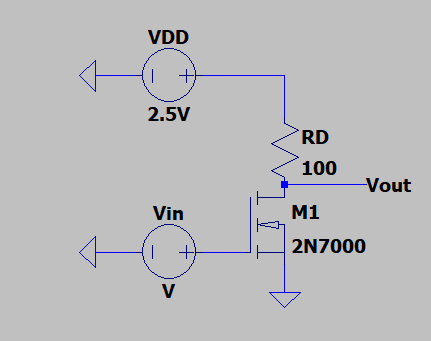
\includegraphics[width = .7\textwidth]{LTspice.png}}
        \end{center}
        \bigbreak
        \item Attach a photo of your physical circuit for $R_D = 100\Omega$ (Follow the instructions in the lab assignment)
\begin{center}
   \boxed{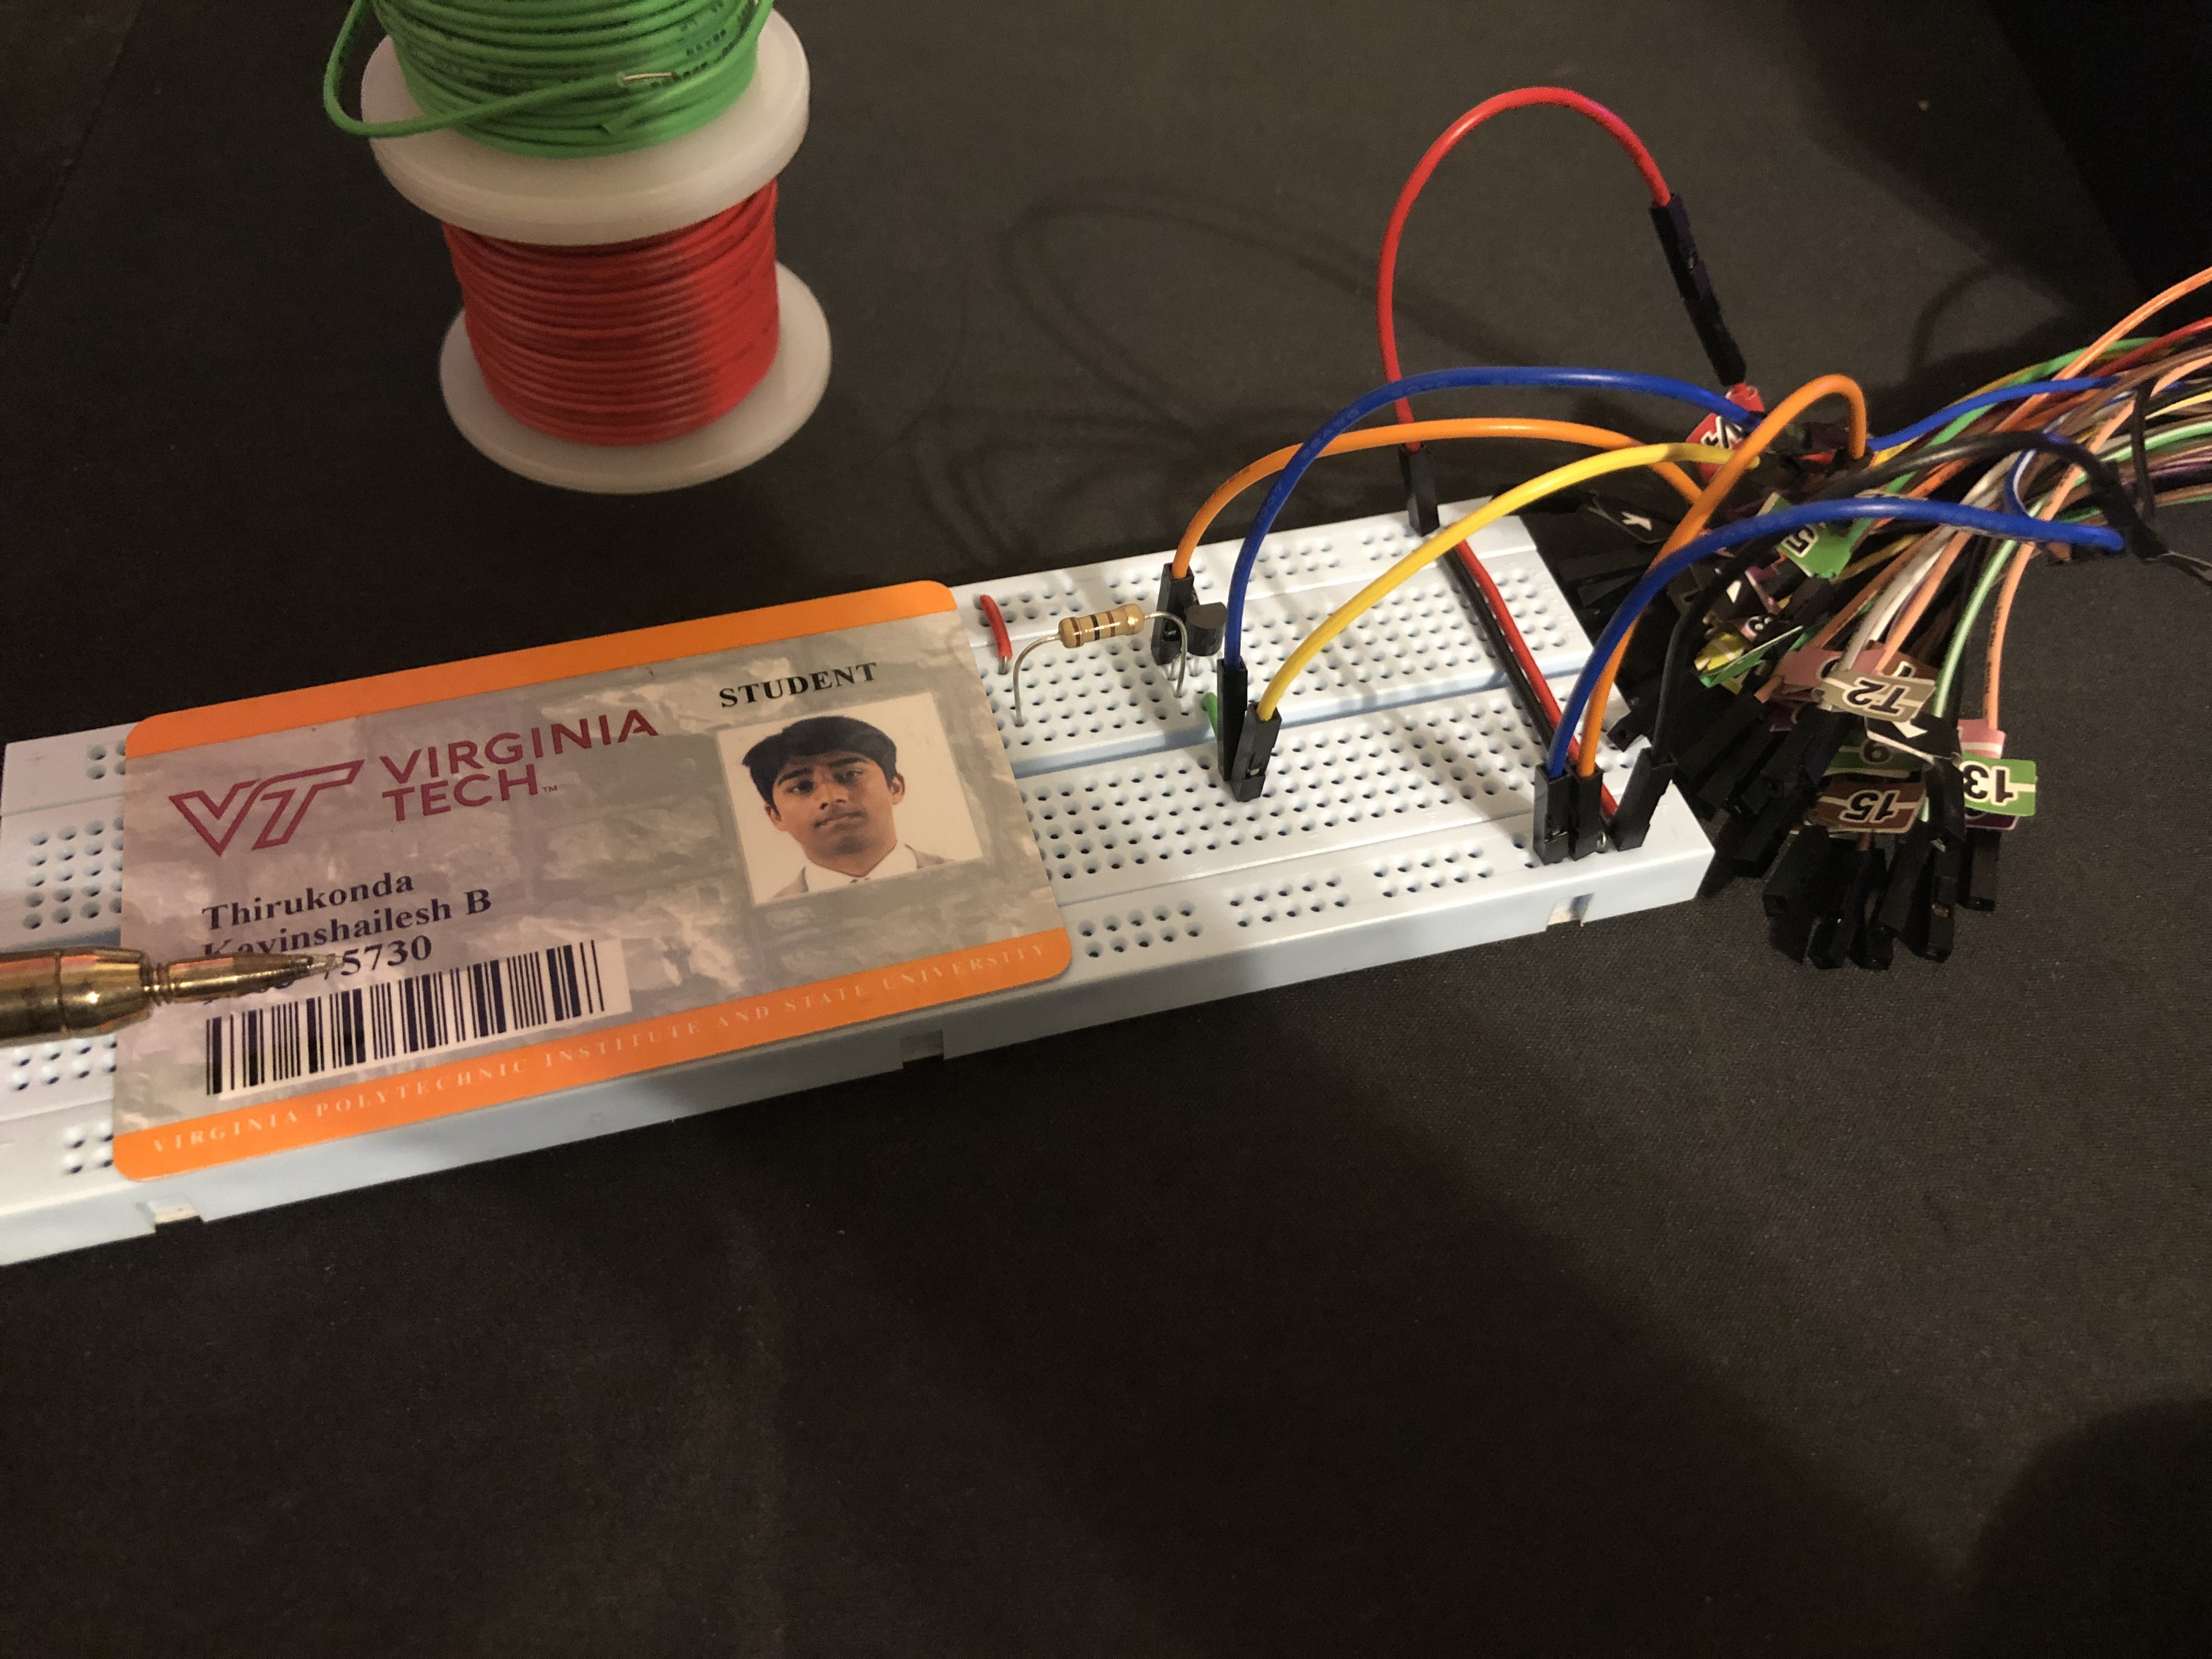
\includegraphics[width = .9\textwidth]{phys.jpg}}
\end{center}
    \end{enumerate}
    \newpage
    \item Simulated vs Physical circuit, $R_D = 100\Omega$.
    \begin{enumerate}
        \item Plot $V_{out}$ for $0V < V_{in} < 2.5V$ of the simulated AND physical circuit for $R_D = 100\Omega$ in the same graph.
        \begin{center}
            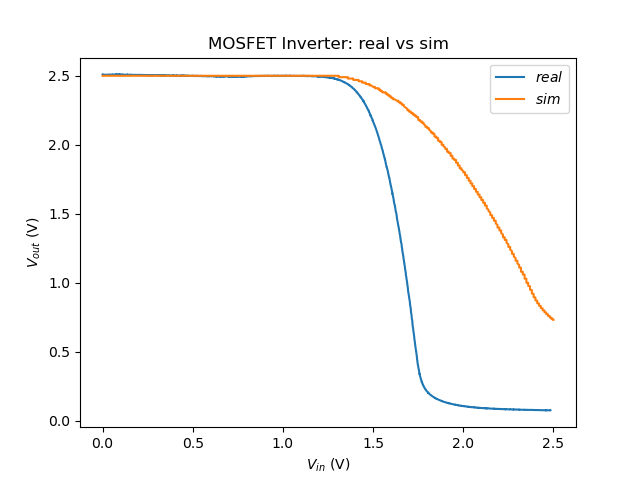
\includegraphics[width = .6\textwidth]{2a.png}
        \end{center}
        \item Compare the voltage transfer curves of the simulated and physical circuits in 2a. Which parameters(s) would you change to make the simulation match more closely?
        \begin{center}
            Some parameters that could be changed are bringing the $K_n$ value up, moving the $V_{TN}$ value down, and most effectively, though it wouldn't make much sense, you could also move the value of $R_D$ up but that would make the two circuits different and wouldn't be plausible for modeling the transistor only the specific circuit.
        \end{center}
    \end{enumerate}
    \item Resistive inverter vs CMOS, physical only.
    \begin{enumerate}
        \item Plot $V_{out}$ of physical circuit for $R_D = 100\Omega, R_D = 50k\Omega,$ and CMOS inverter in the same graph.
        \begin{center}
            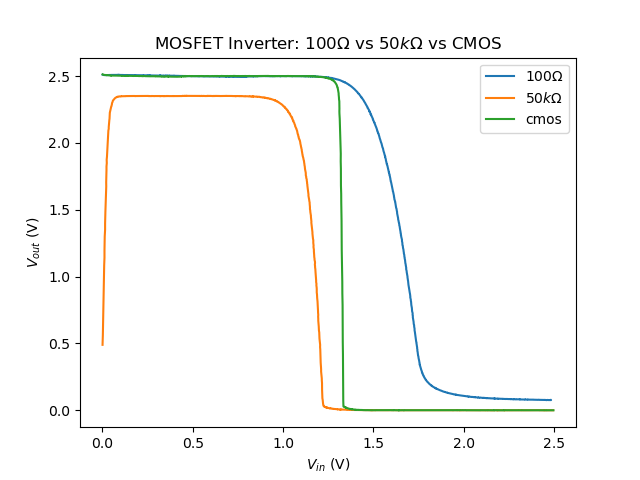
\includegraphics[width = .6\textwidth]{3a.png}
        \end{center}
        \item Compare the three inverter types plotted in 3a: low $R_D$, high $R_D$, and CMOS. Which one performs the best as an inverter, and why?
        \begin{center}
            The CMOS inverter is the clear choice in this situation, while the $50k\Omega$ resitive inverter is slightly more centered which is a benefit, it also has some problems with not reaching max amplitude and for a very small period of time, a voltage of zero will not be inverted. Which makes the CMOS the best option of the three inverters.
        \end{center}
    \end{enumerate}
\end{enumerate}
\end{document}
